\documentclass{article}
\usepackage[parfill]{parskip}
\usepackage{adjustbox}
\usepackage{listings}
\usepackage{graphicx}
\usepackage{color}
\usepackage{hyperref}
\usepackage{tikz}
\usetikzlibrary{shapes.geometric, arrows, positioning}
\tikzstyle{startstop} = [rectangle, rounded corners, minimum width=3cm, minimum height=1cm,text centered, draw=black, fill=red!30]
\tikzstyle{io} = [trapezium, trapezium left angle=70, trapezium right angle=110, minimum width=3cm, minimum height=1cm, text centered, draw=black, fill=blue!30]
\tikzstyle{process} = [rectangle, minimum width=3cm, minimum height=1cm, text centered, draw=black, fill=orange!30, text width=3cm]
\tikzstyle{decision} = [diamond, minimum width=3cm, minimum height=1cm, text centered, draw=black, fill=green!30]
\tikzstyle{arrow} = [thick,->,>=stealth]
\hypersetup{
	colorlinks,
	citecolor=black,
	filecolor=black,
	linkcolor=black,
	urlcolor=black
}
\graphicspath{ {img/} }

\lstset{basicstyle=\ttfamily,
  mathescape=true,
  escapeinside=||}

\begin{document}
\title{COMP33711 - Agile Software Engineering}
\author{Christopher Williamson}
\maketitle
\tableofcontents
\newpage
\section{Introduction}
`We are uncovering better ways of developing software by doing it and helping others to do it. Through this work we have come to value:
\begin{itemize}
	\item \textbf{Individuals and interactions} over processes and tools.
	\item \textbf{Working software} over comprehensive documentation.
	\item \textbf{Customer collaboration} over contract negotiation.
	\item \textbf{Responding to change} over following a plan.
\end{itemize}
That is, while there is value in the items on the right, we value items on the left more.'
\subsection{Key Ideas for Agile Approaches}
One of the key ideas is to avoid waste which commits people to delivering real value. Trust is also a key idea. This includes having a self-organising team, empowering developers to make key decisions and including the customer as a member of the team. Simplicity of both the process and product is important. YAGNI (You Aren't Gonna Need It) is a principle that is often followed which basically means that a programmer should not add functionality until deemed necessary.

Finally, feedback is another key idea. We should aim to `fail fast' by making sure that failure is visible quickly. Short iteration, close customer involvement in development, team retrospectives, high-coverage automated test suites and pair programming are all useful idea that aid the feedback process.

\subsection{12 Agile Principles}
To help people gain a better understanding of what agile software development is all about, the members of the agile alliance refined the philosophies captured in their manifesto into a collection of twelve principles:
\begin{enumerate}
	\item Our highest priority is to satisfy the customer through early and continuous delivery of valuable software.
	\item Welcome changing requirements, even late in development. Agile processes harness change for the customer's competitive advantage.
	\item Deliver working software frequently, from a couple of weeks to a couple of months, with a preference to the shorter time scale.
	\item Business people and developers must work together daily throughout the project.
	\item Build projects around motivated individuals. Give them the environment and support they need, and trust them to get the job done.
	\item The most efficient and effective method of conveying information to and within a development team is face-to-face conversations.
	\item Working software is the primary measure of progress.
	\item Agile processes promote sustainable development. The sponsors, developers, and users should be able to maintain a constant pace indefinitely.
	\item Continuous attention to technical excellence and good design enhances agility.
	\item Simplicity - the art of maximising the amount of work not done - is essential.
	\item The best architectures, requirements, and designs emerge from self-organising teams.
	\item At regular intervals, the team reflects on how to become more effective, then tunes and adjusts its behaviour accordingly.
\end{enumerate}

\subsection{N Agile Practices}
There is no limit on agile practices but some examples are short iterations, user stories, story points, planning games and TDD.

\subsection{M Agile Methodologies}
As above, there is no limit on agile methodologies but some examples are eXtreme Programming (XP), Scrum and Crystal.

\subsection{Waterfall VS Agile}
When using the waterfall approach, we usually have the following structure:\\\\
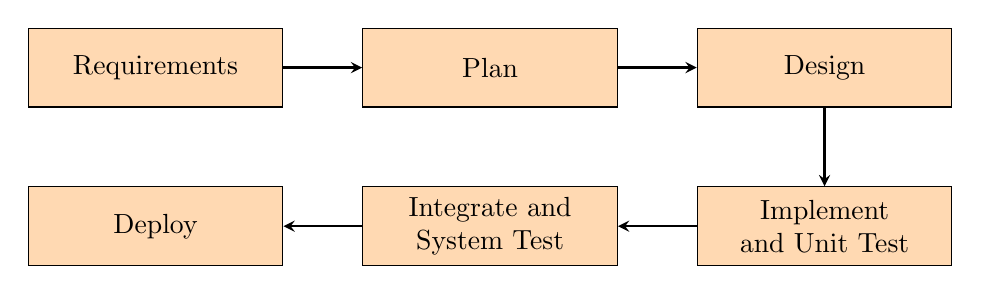
\begin{tikzpicture}[node distance=1cm]
	\node (reqs) [process] {Requirements};
	\node (plan) [process, right= of reqs] {Plan};
	\node (design) [process, right=of plan] {Design};
	\node (unittest) [process, below=of design] {Implement and Unit Test};
	\node (systemtest) [process, left=of unittest] {Integrate and System Test};
	\node (deploy) [process, left=of systemtest] {Deploy};

	\draw [arrow] (reqs) -- (plan);
	\draw [arrow] (plan) -- (design);
	\draw [arrow] (design) -- (unittest);
	\draw [arrow] (unittest) -- (systemtest);
	\draw [arrow] (systemtest) -- (deploy);
\end{tikzpicture}
\newpage
When using the agile approach, our diagram looks like this:\\\\
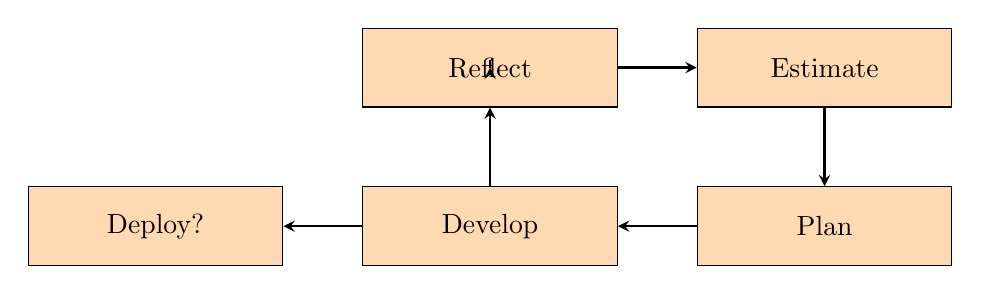
\begin{tikzpicture}[node distance=1cm]
	\node (reqs) [process] {Requirements};
	\node (est) [process, right=of reqs] {Estimate};
	\node (plan) [process, below=of est] {Plan};
	\node (develop) [process, left=of plan] {Develop};
	\node (reflect) [process, above=of develop] {Reflect};
	\node (deploy) [process, left=of develop] {Deploy?};

	\draw [arrow] (reqs) -- (est);
	\draw [arrow] (est) -- (plan);
	\draw [arrow] (plan) -- (develop);
	\draw [arrow] (develop) -- (reflect);
	\draw [arrow] (reflect) -- (reqs);
	\draw [arrow] (develop) -- (deploy);
\end{tikzpicture}\\\\
This diagram shows that the process is iterative and incremental as we loop back to the start (with a reflection stage) at the end of every development cycle (iteration).
\subsection{Iteration Stages}
\subsubsection{Agile Practices: User Stories}
Agile takes a different approach to requirements gathering. Instead of using a typical requirements specification, requirements are gathered as `user stories'.
\begin{center}
	\includegraphics[scale=0.5]{user-story.png}
\end{center}
\subsubsection{Estimation}
You are given a set of user stories. Before starting to build, you need to decide what to commit to.
\subsubsection{Planning}
Next, you select the stories from your backlog that you will implement in the iteration. The key here is balancing business value achieved, effort expended, dependencies between stories and the amount of learning gained from implementation effort. Documenting the plan can be done by using a task board.
\subsubsection{Development and Showcase}
Next you implement as many of your selected stories as you can and show the customer what you've achieved. The customer will sign off the stories that have been completed satisfactorily and the rest will be put into the backlog for the next iteration.
\subsubsection{Feedback}
Finally we hit the feedback stage where we receive feedback from both the customer and the development team in the hope that the feedback will improve out process for the next iteration.

\section{The Trouble with Big Upfront Requirements Gathering}
\subsection{Advantages of a BUFR Specification}
\begin{itemize}
	\item Means that the initial requirements can be put into a contract so that the customer is tied to them.
	\item As the requirements won't change, you can work out how much it'll cost and how much time it'll take to build.
\end{document}
These advantages are based on some assumptions:
\begin{itemize}
	\item There exists a reasonably well-defined set of requirements if we only take the time to understand them.
	\item Changes to requirements will be small enough that we can manage them without substantially rethinking or revising our plans.
	\item Software innovation and the research and development that is required to create a significant new software application can be done on a predictable scale.
\end{itemize}
If all of these assumptions hold it should be fine to proceed with big upfront requirements gathering.
\subsection{Change in Software Requirements}
What can cause requirements to change?
\begin{itemize}
	\item The customer can change the budget.
	\item They don't know what they want through the whole process.
	\item The scale of the project may change.
	\item There may be a big technology change.
\end{itemize}
Given these, there is one major source of change that is often unacknowledged. Changes can occur even on projects where the requirements are not very volatile when the change is in our understanding (customer \& developers) of what the requirements are as we build the system.
